\documentclass[E:/Latex/ExtraWork/ComputerArchitechture/Report.tex]{subfiles}
\usepackage[utf8]{inputenc}
\PassOptionsToPackage{english, british}{babel}
\usepackage[english, british]{babel}
\usepackage{graphicx}
\graphicspath{{../ComputerArchitechture/Chapter3/Figure/}}
\usepackage{amsmath}
\usepackage{amsfonts}
\usepackage{multirow}
\usepackage{booktabs}
\usepackage{indentfirst}
\usepackage{tabularx}
\usepackage{amssymb}
\usepackage{setspace}		%use \doublespacing
\usepackage{svg}
\setsvg{
    inkscape = inkscape -z -D % conversion options for svg package, export drawing instead of page
}
\begin{document}
	\begin{otherlanguage}{english}
		\chapter{Thiết kế CPU RICSV 32 Pipeline 5 tầng}
			\section{Tổng quát về Pipeline }
			\textbf {Pipeline} là một kỹ thuật mà trong đó các lệnh được thực thi theo kiểu chồng lấn lên nhau (overlap).


			Dựa trên thiết kế của đơn chu kỳ ta thấy rằng, để thực hiện một câu lệnh cần ít nhất 5 trạng thái. Các trạng thái được nêu chi tiết trong bảng sau:

			\begin{table}[!ht]
			\begin{tabular}{|l|l|l|l|l|}
			\hline
			IF                                                          & ID                                                                                & EX                                                                    & MEM           & WB         \\ \hline
			\begin{tabular}[c]{@{}l@{}}Instruction\\ Fetch\end{tabular} & \begin{tabular}[c]{@{}l@{}}Instruction\\ decode/register\\ file read\end{tabular} & \begin{tabular}[c]{@{}l@{}}Execute/Address\\ calculation\end{tabular} & Memory access & Write back \\ \hline
			Nạp lệnh                                                    & Decode                                                                            & Tính toán                                                             & Truy cập MEM  & Ghi vào RD \\ \hline
			\end{tabular}
			\end{table}

			\section{Pipelining Hazards}
			\subsection{Structural Hazard}
			Hai câu lệnh cùng truy cập vào bank thanh ghi cùng lúc nhưng nó chỉ có thể đọc hoặc ghi dựa vào Clock.
					\begin{figure}[h!]
						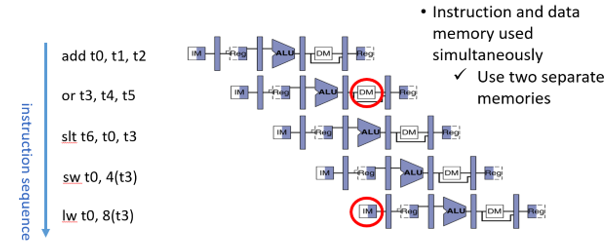
\includegraphics[scale = 1]{Figure/Fig1.png}
						\centering
					\end{figure}
			\newpage		
			\subsection{Control Hazard }
			Hazard control sẽ xảy ra khi dùng các lệnh nhảy như beq, bne,... Sau khi lệnh nhảy đến tầng ALU nhưng địa chỉ kế tiếp chứa câu lệnh thực hiện kế tiếp không biết là nhảy hay không nhảy và nhảy đến đâu
					\begin{figure}[h!]
						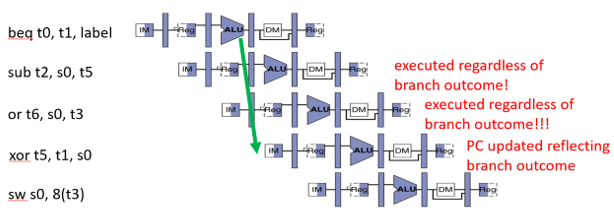
\includegraphics[scale = 1]{Figure/Fig2.png}
						\centering
					\end{figure}
			\subsection{Data hazard }
			Có hai loại Data Hazard 
			\begin{itemize}
				\item \textbf {Hazard R type instruction}
					
					Ở đây ta dùng phương pháp Forwarding để lấy giá trị ở các tầng khác đưa về tầng đang cần dùng giá trị đó. Cấu trúc như sau:
					\begin{figure}[h!]
						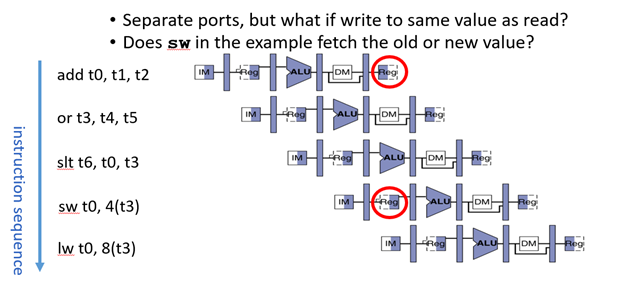
\includegraphics[scale = 1]{Figure/Fig3.png}
						\centering
					\end{figure}
					\newpage
					Việc Forward này có tác dụng đưa các giá trị cần dùng về tầng X khi ở tầng X cần dùng kết quả được tính trong cùng một thanh ghi nhưng nó vẫn chưa Writeback được về băng thanh ghi, ở đây ta cí thể có hai vị trí Writeback về đó là ở tầng M và tầng W. Việc Forward này đều có thể xảy ra được trên cả rs1 và rs2. 
				\item \textbf {Load data hazard}
					\begin{figure}[h!]
						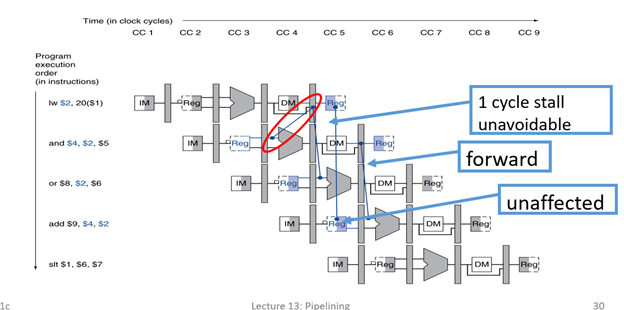
\includegraphics[scale = 1]{Figure/Fig4.png}
						\centering
					\end{figure}

					Lỗi ở đây là việc khi dùng lệnh load vào một thanh ghi nào đó nếu tại thời điểm đó mà cũng chính là thời điểm bộ ALU cần giá trị của thanh ghi đó để tính toán nên ta phải dừng quá trình này lại 1 chu kỳ hay chèn một lệnh NOP vào giữa hai lệnh đó.

					\begin{figure}[h!]
						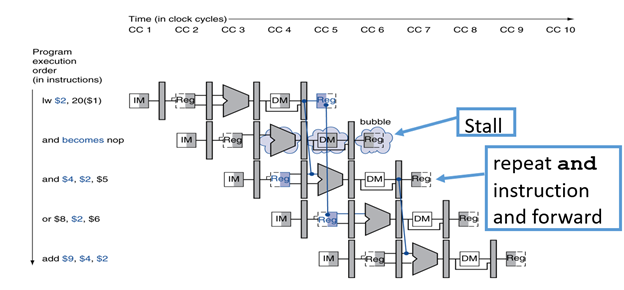
\includegraphics[scale = 1]{Figure/Fig5.png}
						\centering
					\end{figure}
					\newpage
				\section{Thiết kế Pipeline 5 tầng}

				\textbf {Kết quả phần cứng được thiết kế lại sau khi Pipeline:}
				
					\begin{figure}[h!]
						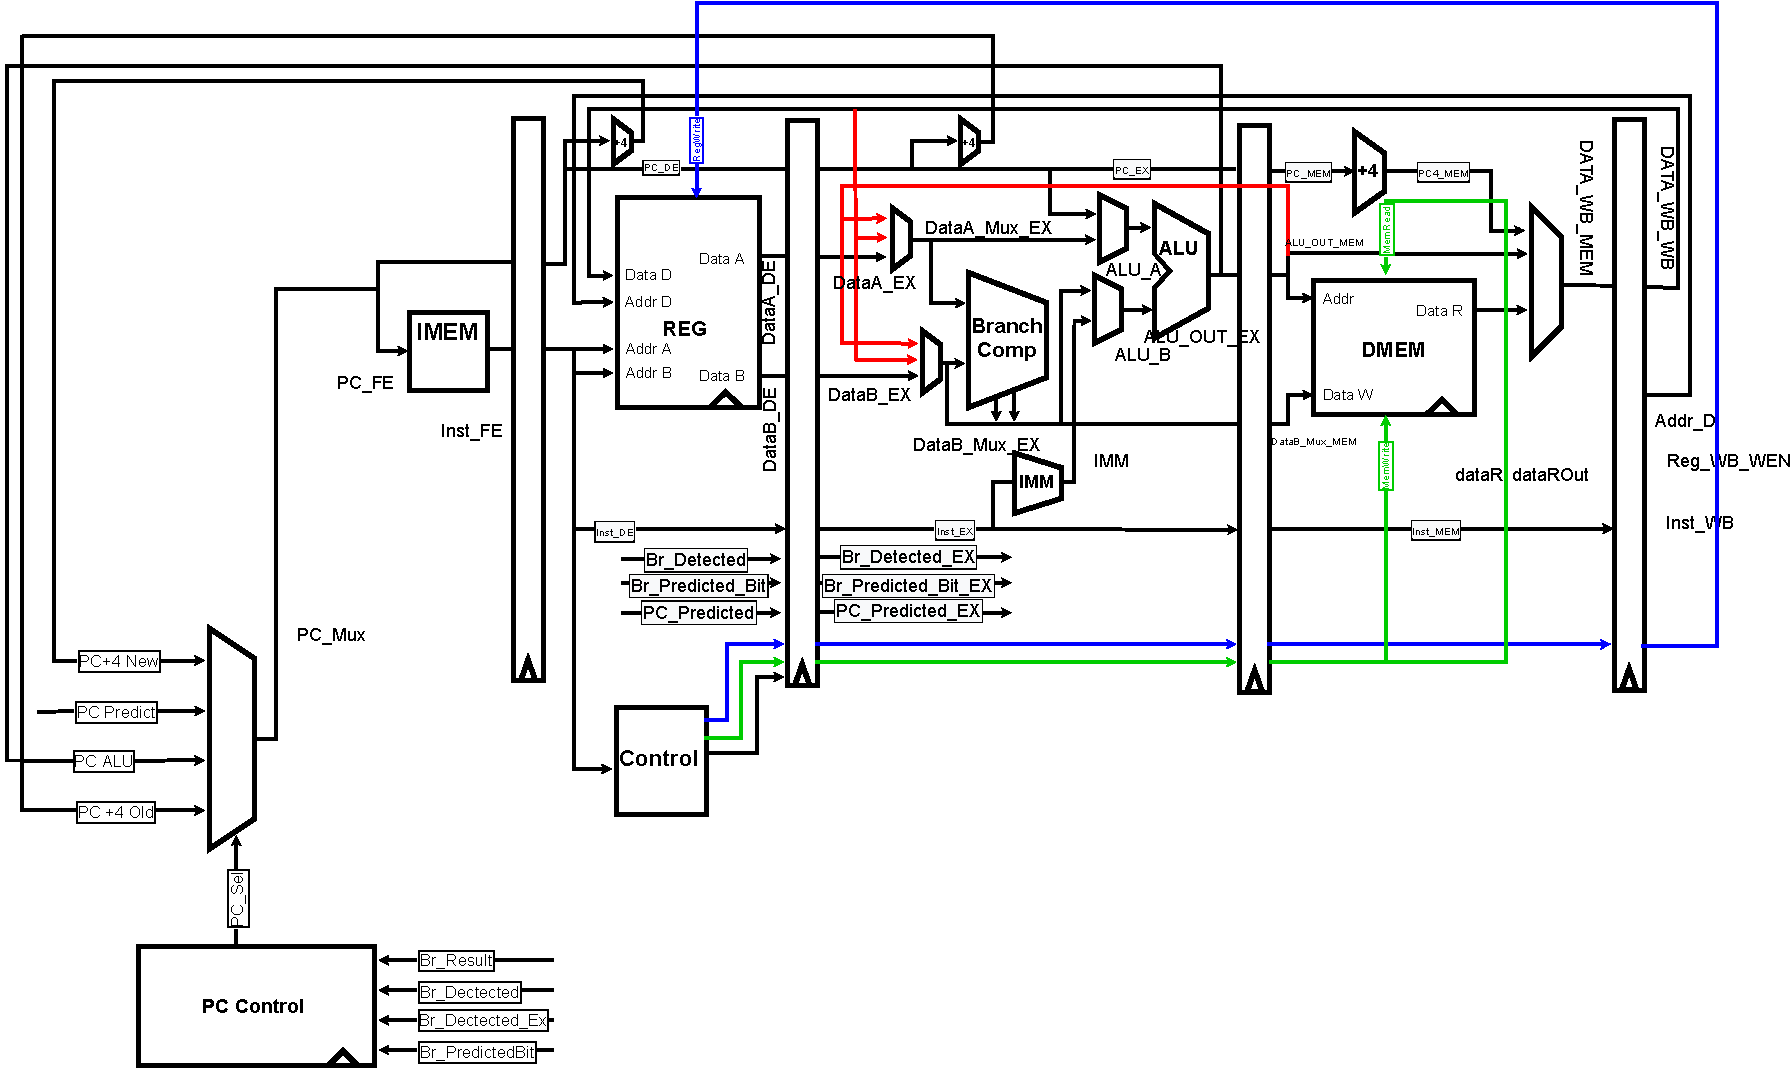
\includegraphics[scale = 0.6]{Figure/pipeline.pdf}
						\centering
					\end{figure}

				\textbf {Ngoài ra, một số khối được thiết kế thêm để giải quyết các vấn đề về Hazard:}
					\begin{itemize}
						\item \textbf {Bộ Stall và Forward}
						\begin{figure}[h!]
							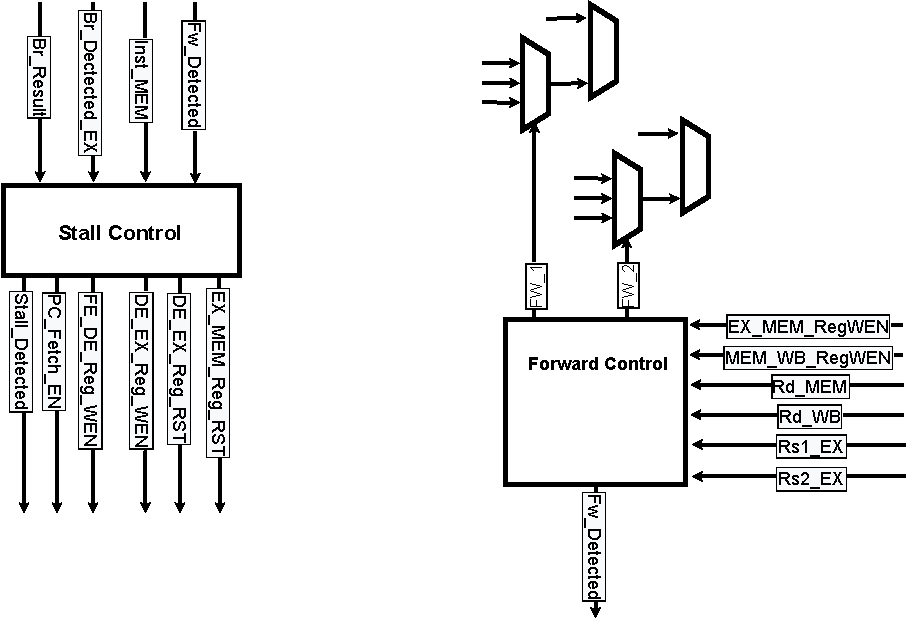
\includegraphics[scale = 0.8]{Figure/S_F.pdf}
							\centering
						\end{figure}

						\newpage
						\item \textbf {Bộ Branch predict}
						\begin{figure}[h!]
							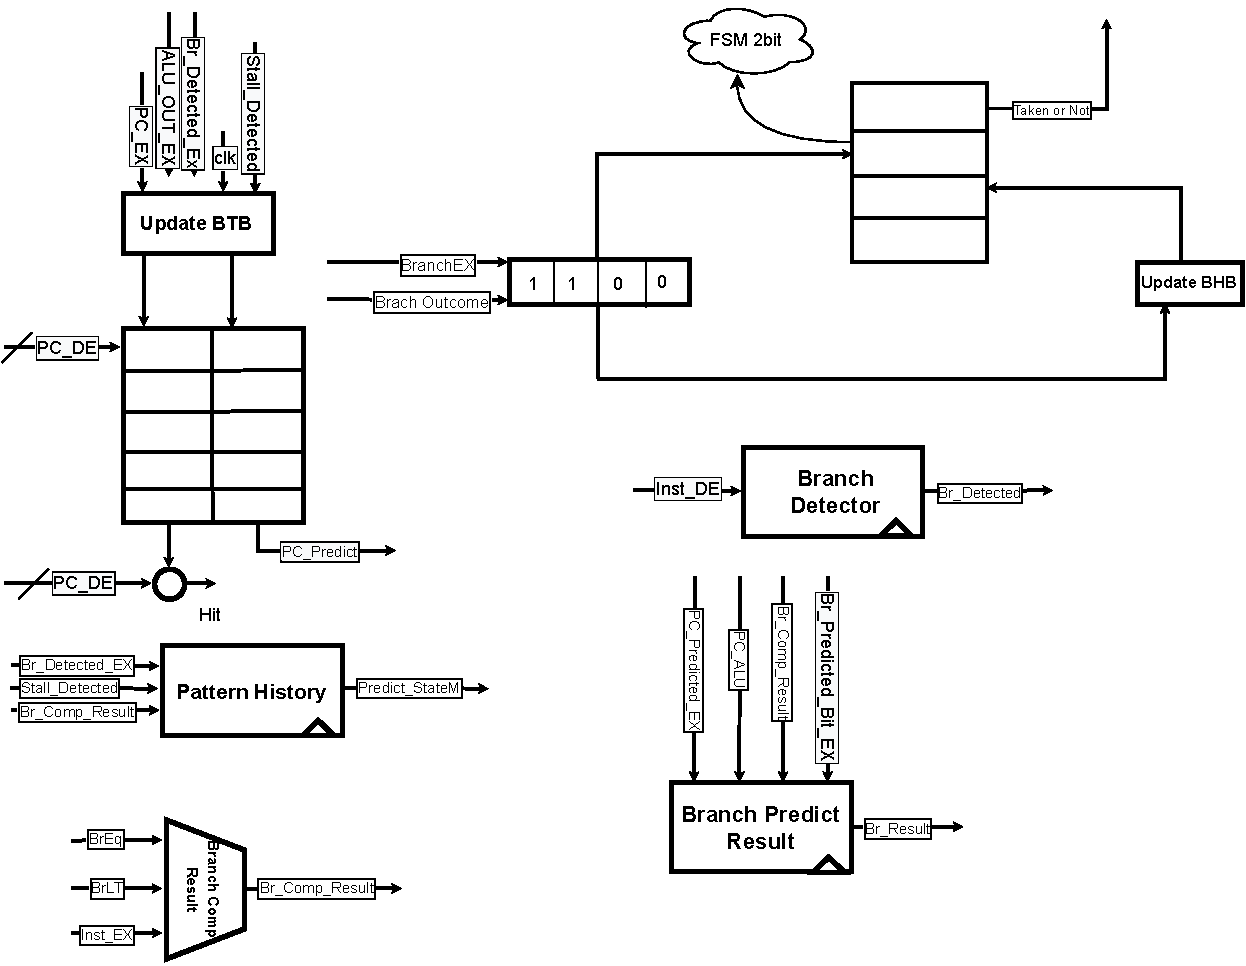
\includegraphics[scale = 0.8]{Figure/Branch.pdf}
							\centering
						\end{figure}	
					\end{itemize}

					
					\section{Thực hiện mô phỏng}
					\subsection{Viết đoạn chương trình test}
						\begin{itemize}
							\item Lấy 10 số lưu trong DMEM và sắp xếp lại rồi lưu vào DMEM ở 10 vị trí tiếp theo.
							\item Tính giai thừa số lớn nhất và lưu ở vị trí tiếp theo.
							\item Tính số Fibonanci của số lớn nhất và lưu ở vị trí tiếp theo.
						\end{itemize}
					
					\newpage
					\subsection{Test dạng sóng trên ModelSim và kết quả mô phỏng}
					Kết quả sau khi chạy đoạn code trên: 
					\begin{figure}[h!]
						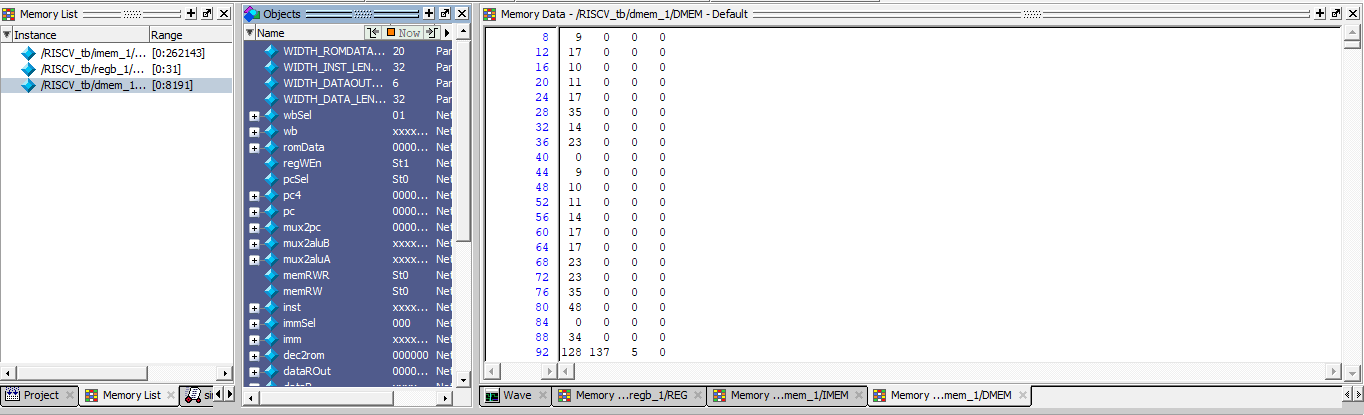
\includegraphics[scale = 0.5]{Figure/Fig6.png}
						\centering
					\end{figure}

					Dạng sóng của đoạn code trên:
					\begin{figure}[h!]
						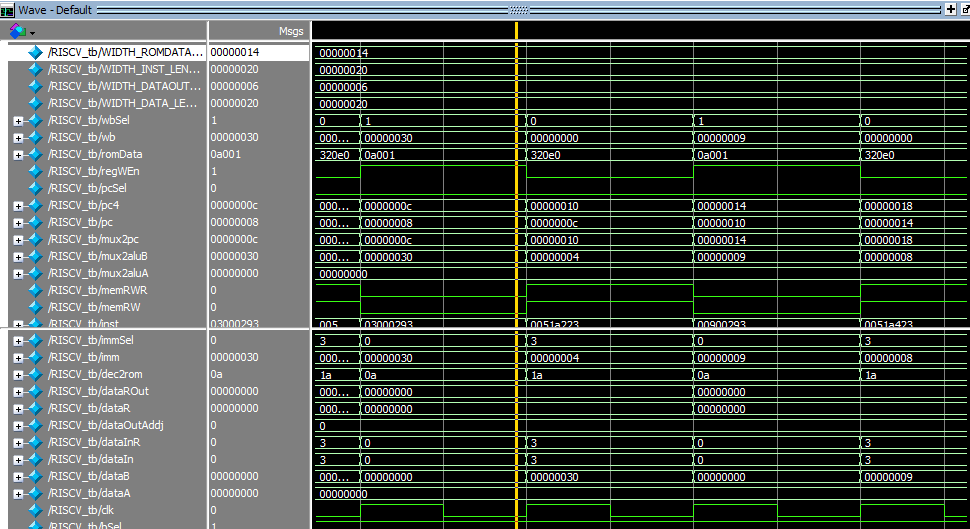
\includegraphics[scale = 0.6]{Figure/Fig7.png}
						\centering
					\end{figure}

			\end{itemize}

	\end{otherlanguage}

\end{document}